\section{Black's ``Leverage'' Effect}

One of the most well-established empirical regularities of equity markets is the negative correlation between the return of stocks and their volatility. In a seminal paper, \cite{Black1976} provides financial leverage as compelling explanation for this phenomenon. While this effect, and the leverage-based explanation, have been empirically confirmed by a number of studies more recent papers show that financial leverage is not the only reason for the negative relation between the return of stocks and their volatility (e.g. \cite{HasanhodzicLo2011}). %For instance, \cite{HasanhodzicLo2011} confirm this negative relation for all-equity financed companies. 
In our model, the negative relation between the stock market return and its volatility is due to the time-variation in consumption/wealth shares.     


We derive the local correlation between stock market returns and changes in stock market volatility in Proposition \ref{prop:LEV}. This correlation is usually set to be negative in the derivatives literature (e.g. \cite{Heston1993}) and it is endogenous in our demand disagreement model. Specifically, we know from the paper that the stock market volatility is strictly increasing in the consumption share until it attains its maximum at $f_{\sigma_R}^{\text{max}}=0.35$ and it is strictly decreasing after that. Positive shocks to the consumption share are good news for the stock market and, thus, the correlation between stock returns and their volatilities is positive for low consumption shares and negative otherwise.  The left plot of Figure \ref{fig:BlackLeverageEffect} provides a graphic illustration of this correlation conditional on the consumption share for different disagreement $\Delta$.  


\begin{prop}[Black's ``Leverage'' Effect]\label{prop:LEV}
Let $f_{\sigma_R}^{\text{max}}$ denote the consumption share value that maximizes the conditional stock market volatility. The local correlation between the return on the stock market and its volatility in equilibrium is
\begin{align}\label{eq:MP_Demand_Sig}
  	\rho_{LE}(f_t) = \text{corr} \left (dR_t, \frac{d\sigma_{R,t}}{\sigma_{R,t}} \right)
  	&= \left \lbrace \begin{array}{lcl}
  		\frac{\sigma^{\alpha}_{R,t}}{\sigma_{R,t}}  
  		& \text{if} & f_t < f_{\sigma_R}^{\text{max}} \\
  		0 & \text{if} & f_t = f_{\sigma_R}^{\text{max}} \\
  		-\frac{\sigma^{\alpha}_{R,t}}{\sigma_{R,t}}  
  		& \text{if} &f_t >f_{\sigma_R}^{\text{max}}. 
  		\end{array} \right. 
\end{align}
\end{prop}
The right graph of Figure \ref{fig:BlackLeverageEffect} shows the unconditional mean of the correlation $\rho_{LE}\left(\tilde{f}\right)$ as a function of disagreement $\Delta$. This correlation is zero without disagreement and becomes negative with low disagreement because in this case there is a low probability of high consumption share realizations of impatient investors. This probability increases when we increase disagreement and, thus, the correlation also decreases for high $\Delta$ after hitting its minimum around $-0.54$.    


\begin{figure}[H]%[htbp]
\centering
\begin{tabular}{cc}
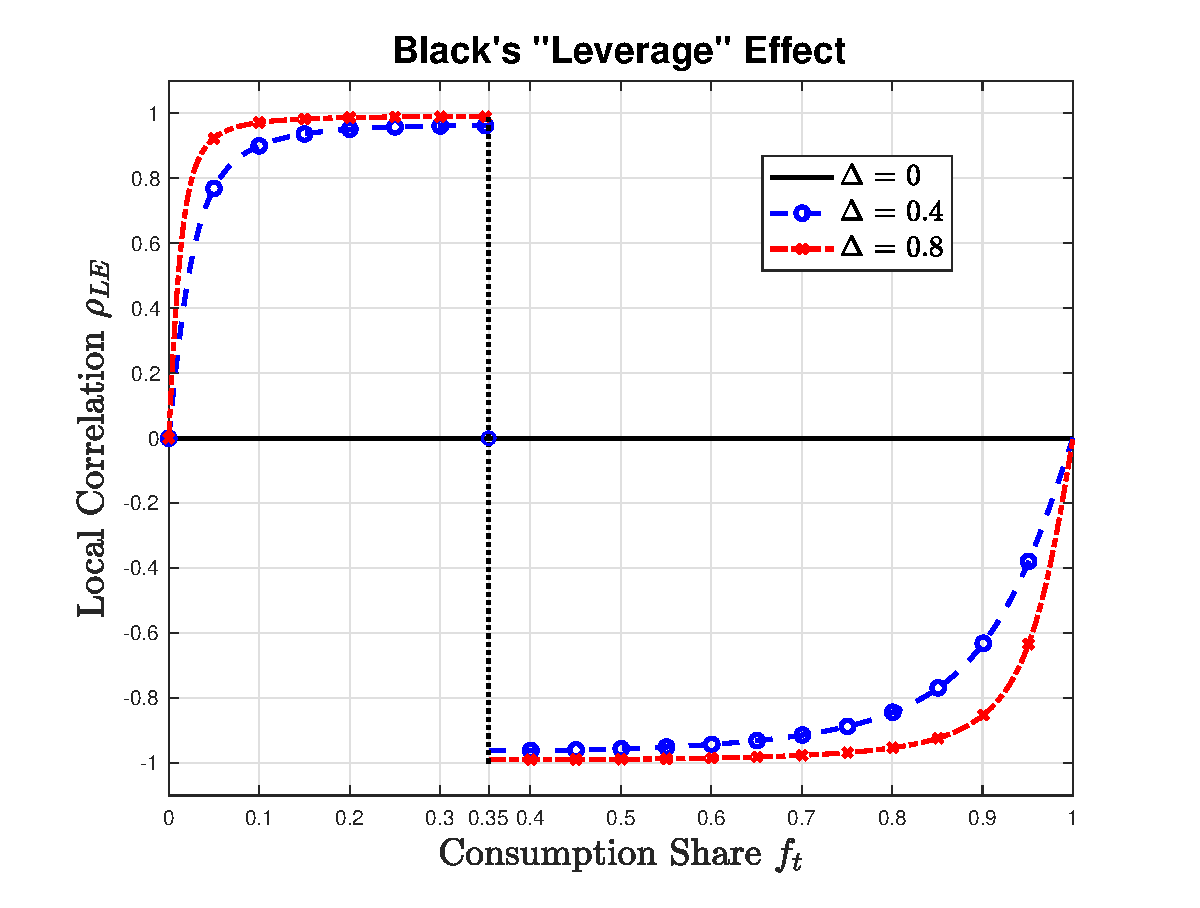
\includegraphics[width=.4\textwidth]{figures/BlackLeverageEffect2f.eps} &  
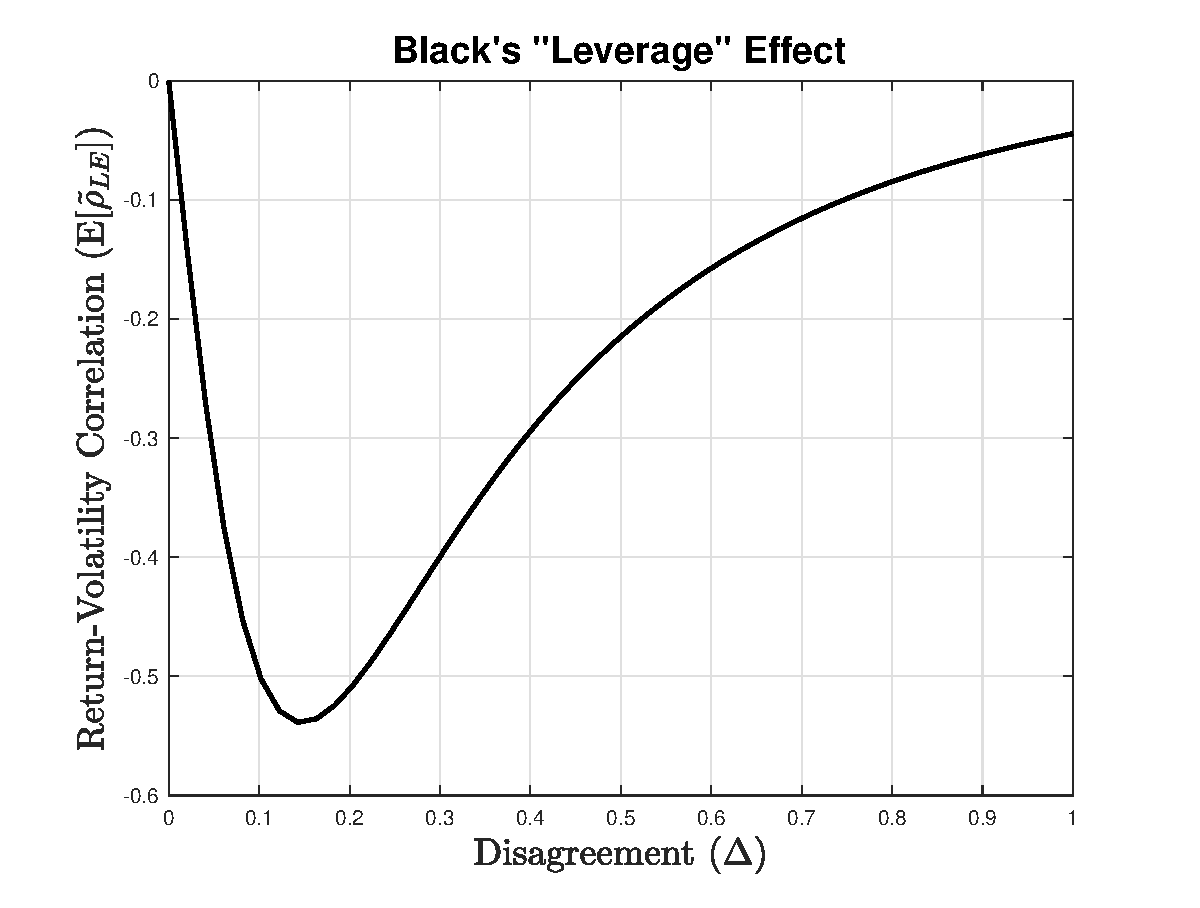
\includegraphics[width=.4\textwidth]{figures/BlackLeverageEffect2DEL.eps} \\ 
\end{tabular}
\caption{\textbf{Black's ``Leverage" Effect.}  \footnotesize{The left graph shows the local correlation between the stock market return and its volatility as a function of the consumption share $f_t$ for different disagreement $\Delta$ and the right graph shows the unconditional distribution of this correlation as a function of disagreement $\Delta$.   The unconditional statistic is based on one million years of monthly observations for each value of disagreement $\Delta$. In this example the parameters are based on the alternative calibration with $\rho^a = 0.001$ and $\rho^b = 0.05$}} 
\label{fig:BlackLeverageEffect} 
\end{figure}


